\section{Hyperspectral Imager (HSI) Payload} \label{sec:hsi}

The HSI design is based on a grating spectrograph (without prism). Components are mainly commercial off-the-shelf from Thorlabs.com and Edmund Optics, except for the grating holder which may be 3D printed. The detector is an industrial camera head from The Imaging Source Europe GmbH. sensor used is the CMOS image sensor Sony IMX249. A 300 grooves/mm transmission grating is blazed at 17.5$^{\circ}$ with efficiency above 50\% for 400-800 nm spectral range. The aperture is 24 mm with an input F/value equal to 2. The input slit width is adjustable with no magnification of the slit height ($\tilde{h}_{\text{slit}}$ = 7.032 mm). A slit width of $w_{\text{slit}}$ = 50 $\mu$m will result in a spectral bandpass (FWHM) of approximately 1.67 nm without binning. Fig. \ref{fig:optics} shows the layout of an optical diagram which visualizes a center cross-section of the instrument, parallel to the refraction axis.
\begin{figure}[htbp]
  \centering
      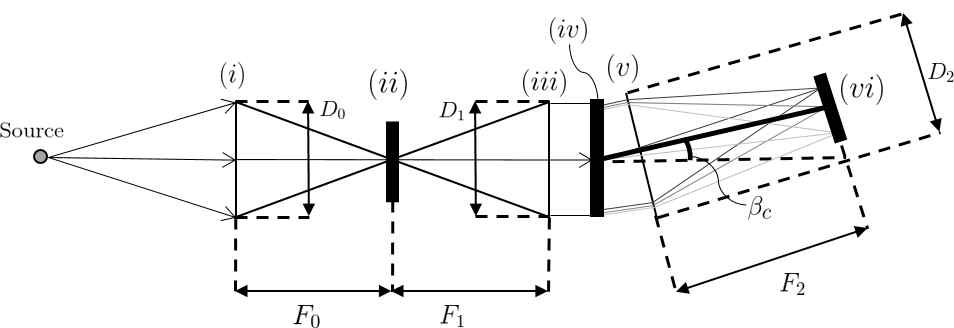
\includegraphics[width=0.5\textwidth]{figs/optics.png}
  \caption{Optical diagram of Spectrometer. $L_0$ is the front lens with lens diameter $D_0$, $f_0$ is the focal length between $L_0$ and entrance slit $S_1$, $B$ is the back focal length, $f_1$ is the focal length between entrance slit $S_1$ and collimator lens $L_1$ with diameter $D_1$, $G$ is the grating with lens $L_2$, $f_2$ is the focal length between the grating $G$ and the detector $X$. The light dispersion angle is $\beta \approx 10.37^{\circ}$. Credit: Fred Sigernes.}
	\label{fig:optics}
\end{figure}
The current HSI V6 prototype (Version 6) is depicted in Figure \ref{fig:hsi}. Further specifications are given in Table \ref{tab:specs} that describe the HSI performance.
\begin{figure}[htbp]
  \centering
      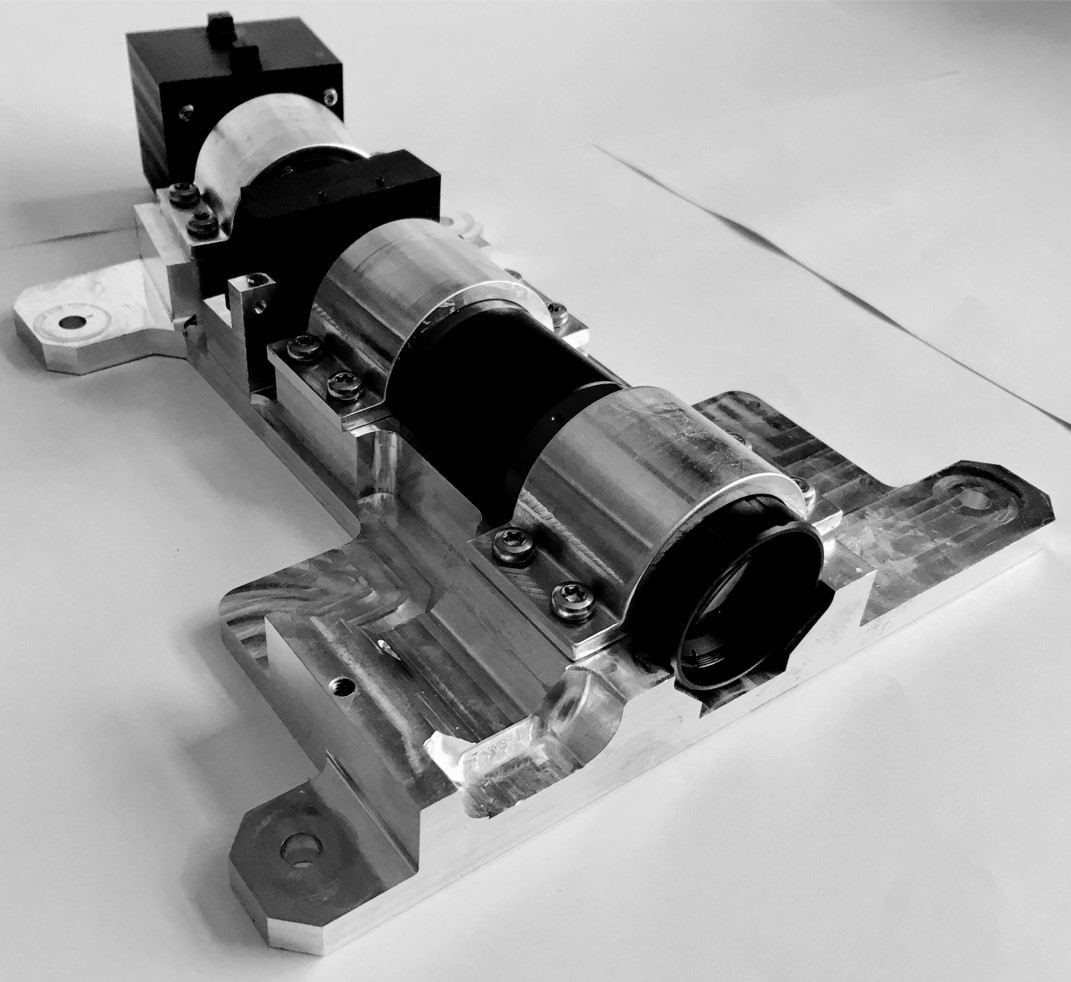
\includegraphics[width=0.5\textwidth]{figs/HSI.png}
  \caption{Current HSI version 6. Credit: Fred Sigernes.}
	\label{fig:hsi}
\end{figure}
\begin{table}[htbp]
	\caption{HSI version 6 Optics Dimensions}
	\label{tab:optics}
	\centering
			\begin{tabular}{p{2cm} p{2cm} l }
				\hline
				Part &	Dimensions & Description   \\
				\hline
				$f_0/\#$ & $f_0/2$ & f-number front lens \\
				$A_0 (L_0)$ & 24 mm & Aperture front lens \\
				$f_0$ & 50 mm & Focal length front lens \\
				$B$ & 8.6 mm & Back-flange focus \\
				$w_{\text{slit}}$ &	50 ${\mu}$m &  Entrance slit width \\
				$h_{\text{slit}}$ &	7 mm  & Entrance slit height \\
				$\tilde{h}_{\text{slit}}$ &	7.032 mm  & Effective entrance slit height \\
				$f_1/\#$ & $f_1/2$ & f-number collimator lens \\
				$A_1 (L_1)$ & 25 mm & Aperture collimator lens \\
				$f_1$ &	50 mm & Focal length collimator \\
				$G$ &	$25\times 25$ mm$^{2}$ & Grating area \\
				$A_2 (L_2)$ & 25 mm & Aperture grating lens \\
				$f_2/\#$ & $f_2/2$ & f-number detector lens \\
				$f_2$ &	50 mm & Focal length detector lens \\
				\hline
				\end{tabular}
\end{table}
\begin{table}[htbp]
	\caption{HSI version 6 Performance Specifications}
	\label{tab:specs}
	\centering
			\begin{tabular}{p{4cm} p{4cm}}
				\hline
				Mass $m$ & 544 g \\
				Volume & $80 \times 60 \times 220 $ mm \\
				$iFoV$ &	$0.0564^{\circ} \times 7.8826^{\circ}$  \\
				Total optical efficiency $\eta_{\text{OE}}$ & $0.8^3 \approx 0.5$ \\
				Grating & 300 grooves/mm \\
				Grating efficiency $\eta_{\text{G}}$ \@500 nm & 73 \% \\
				Sensor Resolution & $1936 \times 1216$ pixels \\
				Spectral range & 400-800 nm \\
				Bandpass $\Delta \lambda$ & 3.34-10 nm \\
				Pixel size $p_x \times p_y$ & $5.86 \mu\text{pixels} \times 5.86 \mu\text{pixels}$\\
				Binning & Up to $10\times$ \\
				Usable bands & 87 \\
				Quantum efficiency $\eta_{\text{QE}}$ \@500 nm & 77 \% \\
				Dark current & 0.95 $e^{-}/s$ \\
				Read-out noise (25 C$^{\circ}$) & 6.93 $e^{-}$ \\
				\hline
				@ altitude $h$ = 500 km, view angle $\theta=0^{\circ}$, and exposure time $\Delta t$ = 25.4 ms & \\
				\hline
				Swath width & 70 km \\
				$\delta x$ & 500 m \\
				$\Delta x$ & 693.65 m \\
				$\Delta y$ & 58.6 m \\
				$v_{\text{sat}}$ &  7.624 km/s\\
				\hline
				\end{tabular}
\end{table}
Table \ref{tab:spectrometer_designs} offers spectrometer designs that are different but may achieve same goals as the HSI version 6. 

\begin{table*}[htbp]
	\caption{Other spectrometer designs}
	\label{tab:spectrometer_designs}
	\centering
			\begin{tabular}{|l|p{12cm}|}
				\hline 
				Type & Description \\
				\hline
				PRISM "Dyson" \cite{Mouroulis2014} & Considered the "best" dark target pushbroom hyperspectral prototype to consider, combining low f-number, low internal scattering, and low monochromatic and chromatic aberrations to maximize SNR over dark targets. \\
				\hline
				Offner \cite{PrietoBlanco2006}  & Three-concentric-mirror (Offner) configuration. The approach presented allows for the rapid design of this class of system. \\
				\hline
				CHAI V-640 \footnote{http://brandywinephotonics.com/2013/05/16/chai-v-640-2/} & Commonly used airborne sensor for validation campaigns for remote sensing (satellite hyperspectral imagery) \\
				\hline
				NovaSol \footnote{https://www.corning.com/worldwide/en/products/advanced-optics/product-materials/spectral-sensing.html} & Airborne hyperspectral design but possibly at larger form factor \\
				\hline
				\end{tabular}
\end{table*}

\subsection{Electronics}
The goal of the PCB is to get the entire processing chain up and running with image sensor and on-board processing, and to get a better understanding of the challenges involved in hyperspectral imager hardware development. The HSI will be mounted on a 9.4$\times$ 9.4 cm PCB with FPGA processing unit for onboard data handling and image processing. The PCB, as shown in Figure \ref{fig:HSI_PCB}, is based on using an ARM/FPGA (Zynq7000) computer and has average power consumption of 3-3.5 W. It also supports multiple protocols across its processors.

\begin{figure}[htbp]
  \centering
      \includegraphics[width=0.35\textwidth]{figs/HSI_PCB.png}
  \caption{PCB developed for the HSI to be mounted at 2.5U in \hypso. The image sensor used here is a CMOSIS CMV2000.}
	\label{fig:HSI_PCB}
\end{figure}

Specifications for the PCB are
\begin{itemize}
\item Storage: 36GB (4GB eMMC + 32GB microSD)
\item Memory: 1GB RAM
\item Processor: Dual Core ARM A9 (Zynq 7030 Series FPGA)
\item Input Voltage: 4.5-14.5V
\item Maximum current: 6A 
\item Connectivity: GiGEthernet
\end{itemize}

The data is read out using low voltage differential singling (LVDS) and controlled using SPI. For maximum quantum efficiency, the variation of the sensor processed on 12 $\mu$m epitaxial (E12) SI wafer is used. The thicker epic-layer increases the sensitivity to light above 600 nm significantly. Due to the sensitivity due to high speed data transfer, the data lines are carefully impedance-matched following the TIA/EIA 644 standard for LVDS signals.

\subsection{Performance}
The spectral bandpass is given as, where $a = 3333.33$ nm is the groove spacing. Spectral order is $k=1$ and incident angle $\alpha$ = 0. If the slit width is $w_{\text{slit}} = 50 \mu$m then $BP= 3.34$ nm. The effective slit height is $\tilde{h}_{\text{slit}}=7.032$ mm. This is the height of the Sony IMX249 CMOS detector.

Since the satellite will be in a sun-synchronous orbit at $h\approx 500$ km altitude, the FoV at Nadir may be calculated as follows:
\begin{equation}
iFoV = \tan{\frac{w_{\text{slit}}}{f_0}} \times \tan{\frac{h_{\text{slit}}}{f_0}}
\end{equation}
giving $iFoV=0.0564^{\circ} \times 7.8826^{\circ}$ (in-track $\times$ cross-track). This results in larger pixels along the direction of flight as compared to lower altitudes, and defines the spatial resolution as illustrated in Fig \ref{fig:spatial}. The distance $\delta x$ defines the ground segment optical resolution as seen by the instrument at time $t = t_0$ and is the instantaneous ground resolution expressed as,
\begin{equation}
\delta x = \frac{h w_{\text{slit}}}{f_0}
\end{equation}
Raw instantaneous sampling is illustrated in Fig \ref{fig:sampling}. The spatial resolution may be calculated as,
\begin{equation}
\Delta x = \delta x + v_{\text{sat}} \Delta t \label{eq:spatial}
\end{equation}
where $\Delta t=t_1-t_0$ is the exposure time and $v_{\text{sat}}$ is the speed of the satellite. It does not include the read-out time $\tau$ for the sensor. The criterion for read-out time may be determined as,
\begin{equation}
\tau \leq \left( \frac{h w_{\text{slit}}}{f_0 v_{\text{sat}}}\right)
\end{equation}
Cross-track to the flight direction the resolution is calculated simply as
\begin{equation}
\Delta y = \frac{h \tilde{h}_{\text{slit}}}{f_0 N_y}
\end{equation}
where $N_y$ is the effective number of pixels along the slit image.

For exposure time of $\Delta t = 25.4$ ms (read-out time should be less than or equal 64.5 ms), 39.56 frames per second ($1/(\Delta t) \approx 39.56$ fps) and the HSI specs $f_0=$50 mm, $w_{\text{slit}}=0.50 \mu$m, $f/2$ and $N_{y}=1200$, this gives $\delta x =$500 m, $\Delta x =$693.65 m, $\Delta y =$58.6 m and swath width $SW=70$ km.

\begin{figure}[htbp]
  \centering
      \includegraphics[width=0.3\textwidth]{figs/spatial.png}
  \caption{FoV of slit as satellite moves with velocity $v_{\text{sat}}$ and $h$ is altitude above ground level. The spatial resolution then becomes equal to the distance from point A to B denoted as $\Delta x$.}
	\label{fig:spatial}
\end{figure}

\begin{figure}[htbp]
  \centering
      \includegraphics[width=0.4\textwidth]{figs/sampling.png}
  \caption{Nadir mapping of $70 \times 70$ km$^{2}$ target area with optical resolution $\delta x = 500$ m.}
	\label{fig:sampling}
\end{figure}

\subsection{Signal-to-Noise Ratio} \label{sec:snr}
This section covers the sensitivity analysis of optics performance to determine feasibility of the sensor and image acquisition from Low-Earth-Orbit (LEO) at $h=500$ km. The methodology is based on relevant calculations from Ocean Optics Website\footnote{\url{http://www.oceanopticsbook.info}} and a RESONON white paper on SNR\footnote{\url{https://www.resonon.com}}. It can be seen in Fig. \ref{fig:sensor1} that significant atmospheric disturbances increases with altitude. Radiances in Wm$^{-2}$sr$^{-1}$nm$^{-1}$ are modeled with the following MODTRAN inputs and assumptions that were run in Hydrolight Software: 
\begin{itemize}
\item cloudless mid-latitude summer atmosphere
\item marine aerosols present
\item relative humidity of 76$\%$ at sea level
\item solar zenith angle of 50$^{\circ}$
\item surface wind speed of $ 6$ m/s
\item Nadir-viewing sensor ($\gamma=0^{\circ}$)
\item horizontal visibility of $63$ km
\item homogeneous water
\item Case 1 water with Chl-a concentration of 1 mg/m$^{-3}$
\item infinitely deep water
\end{itemize} 

\begin{figure}[htbp]
  \centering
      \includegraphics[width=0.5\textwidth]{figs/sensor1}
  \caption{Example generated (from HydroLight software) radiances $L_u$ for different HSI sensor altitudes with Case 1 water and Chl-a concentration of 1 mg/m$^3$ which is pretty low. The water-leaving radiance and surface-reflected radiance (not shown) are the same in all cases. Shows significant atmospheric disturbances with increasing altitude. Reference: \url{http://www.oceanopticsbook.info}}
	\label{fig:sensor1}
\end{figure}

The radiances are re-run in HydroLight software for spectral range of 400-800 nm with spectral resolution of 5 nm in Figure \ref{fig:radiance}. 
\begin{figure}[htbp]
  \centering
      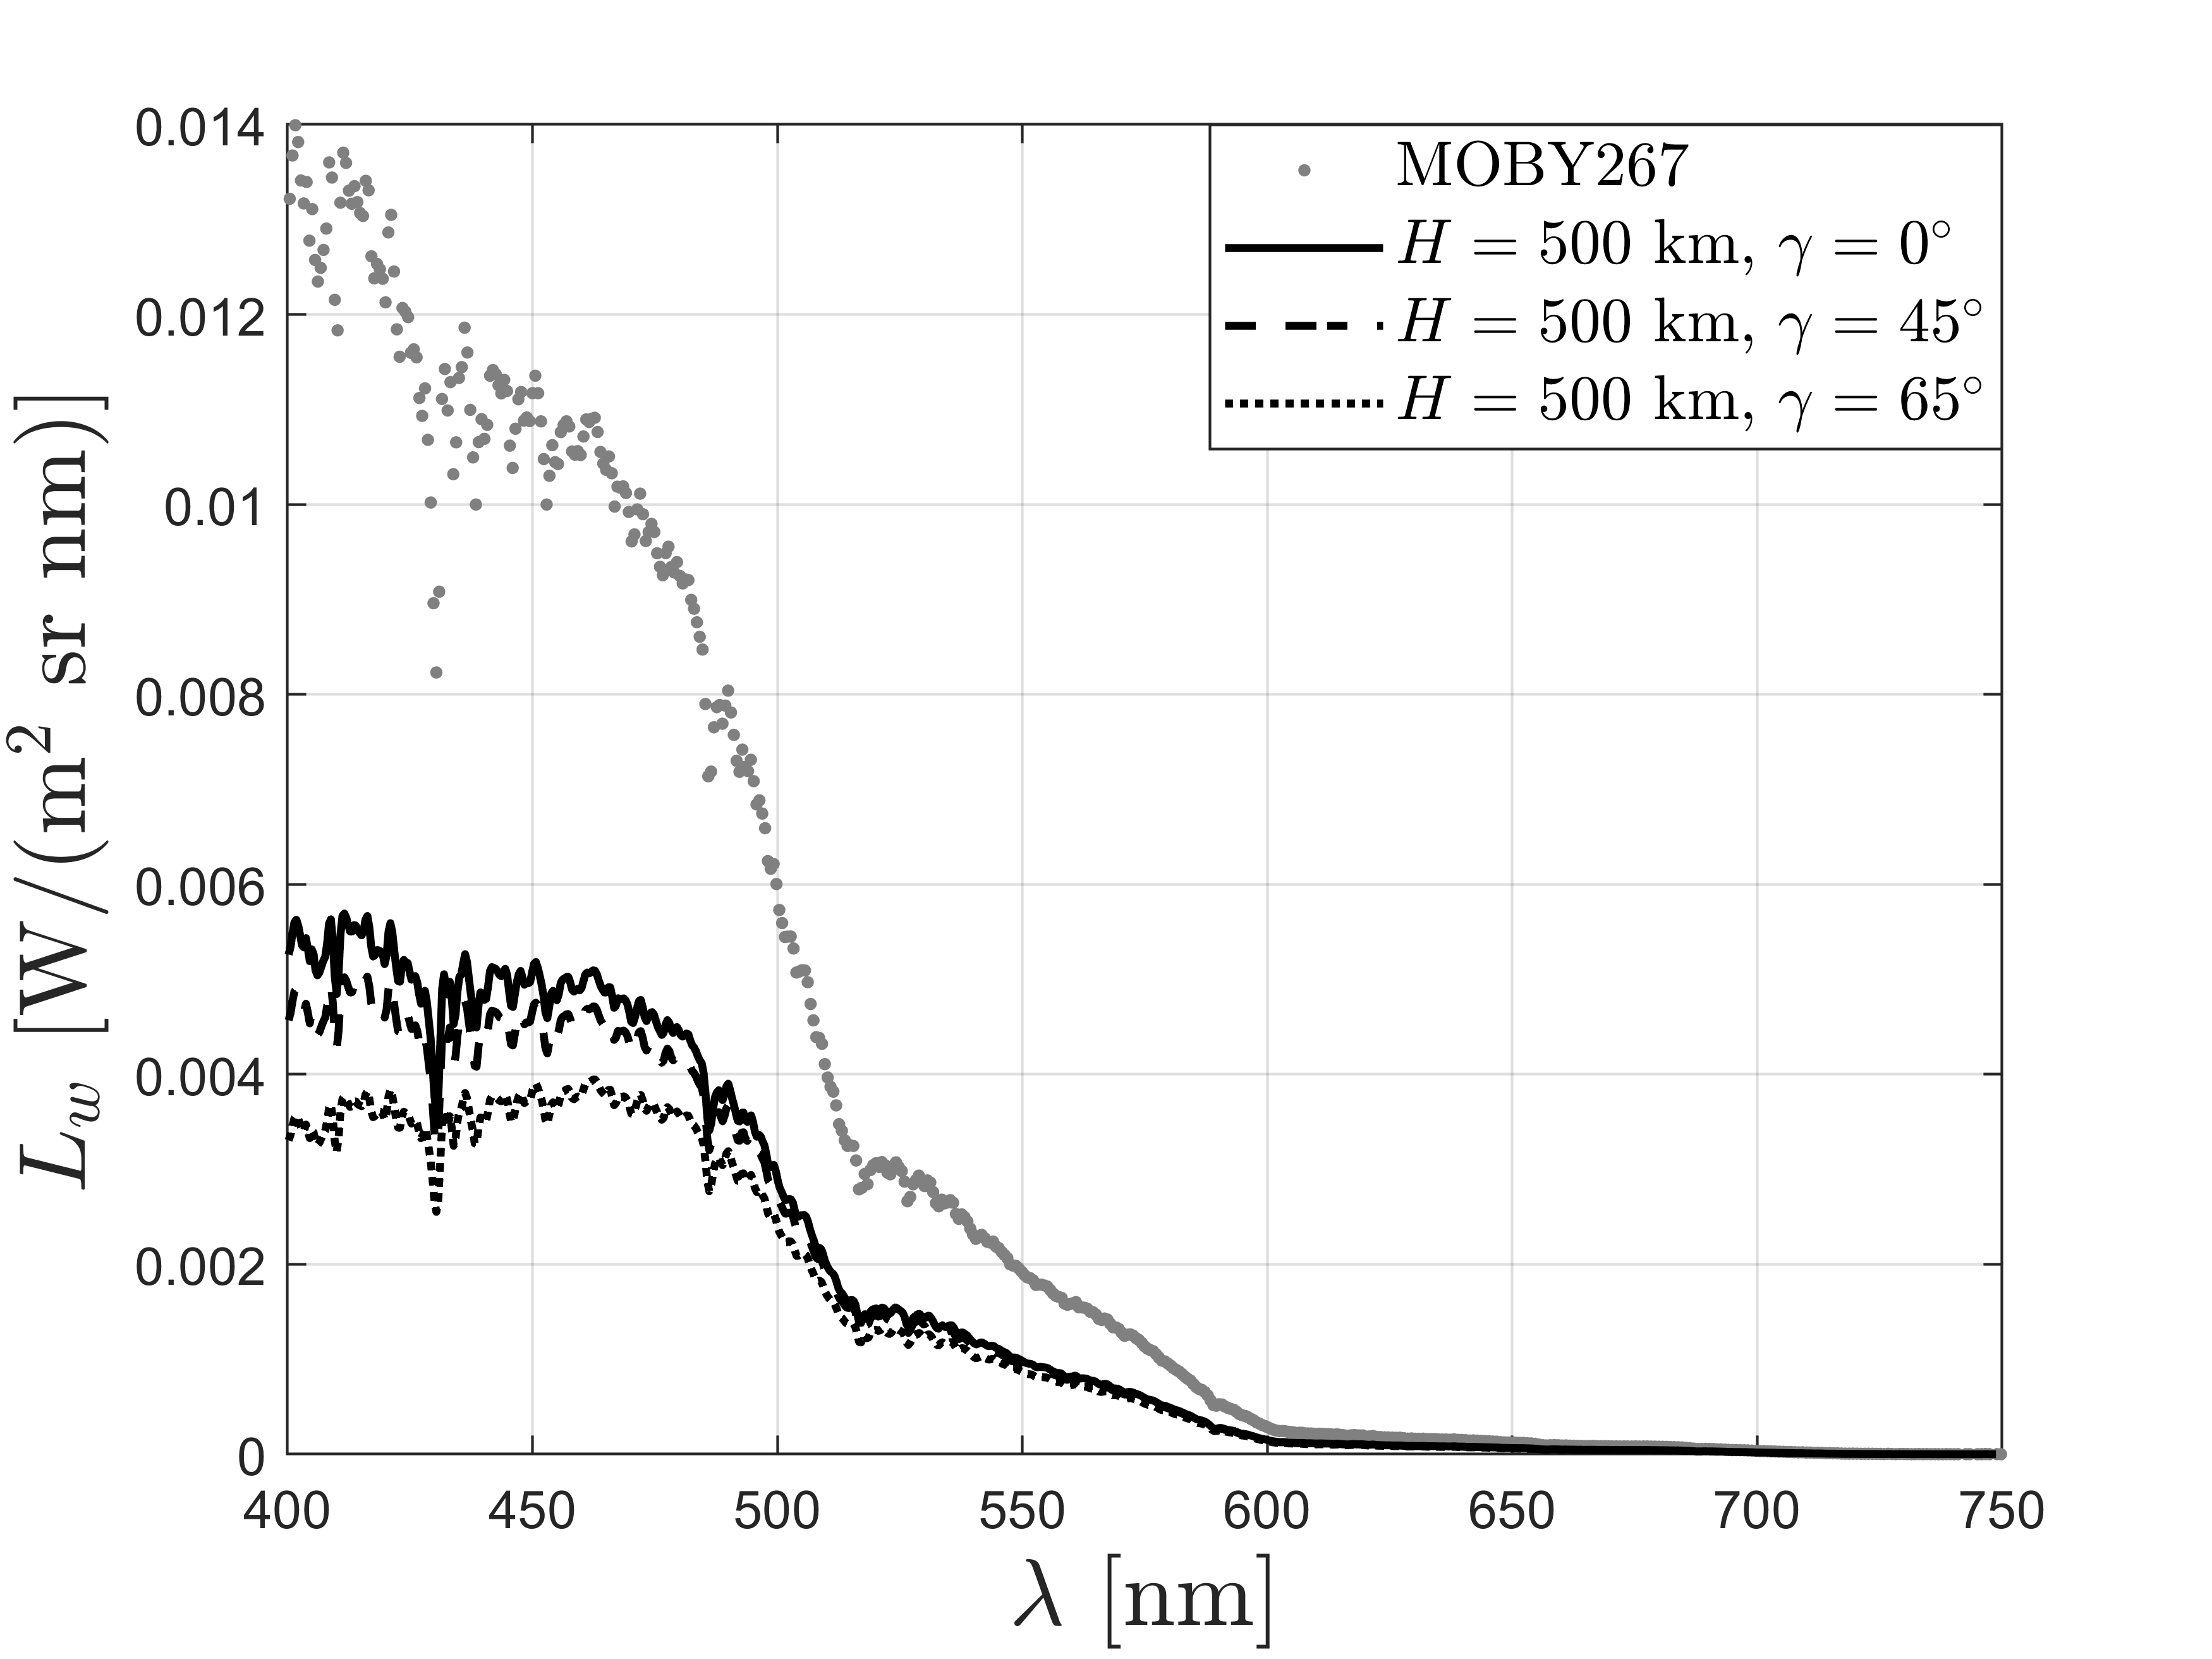
\includegraphics[width=0.5\textwidth]{figs/radiance.png}
  \caption{$L_u$ reaching the HSI sensor in-situ and top of atmosphere (ToA) which determines amount of photons detected at each spectral band with $\Delta \lambda =5$ nm. Reference: \url{http://www.oceanopticsbook.info}.}
	\label{fig:radiance}
\end{figure}

One of the parameters to understand the performance of the camera with respect to a desired signal or photons reaching the sensor is to determine the signal-to-noise ratio (SNR). The constants for the HSI are required to determine photon count as shown in Tables \ref{tab:optics} and \ref{tab:specs}.

The sensor and grating efficiencies at each wavelength are shown in Figure \ref{fig:optical_eff}.
\begin{figure}[H]
  \centering
      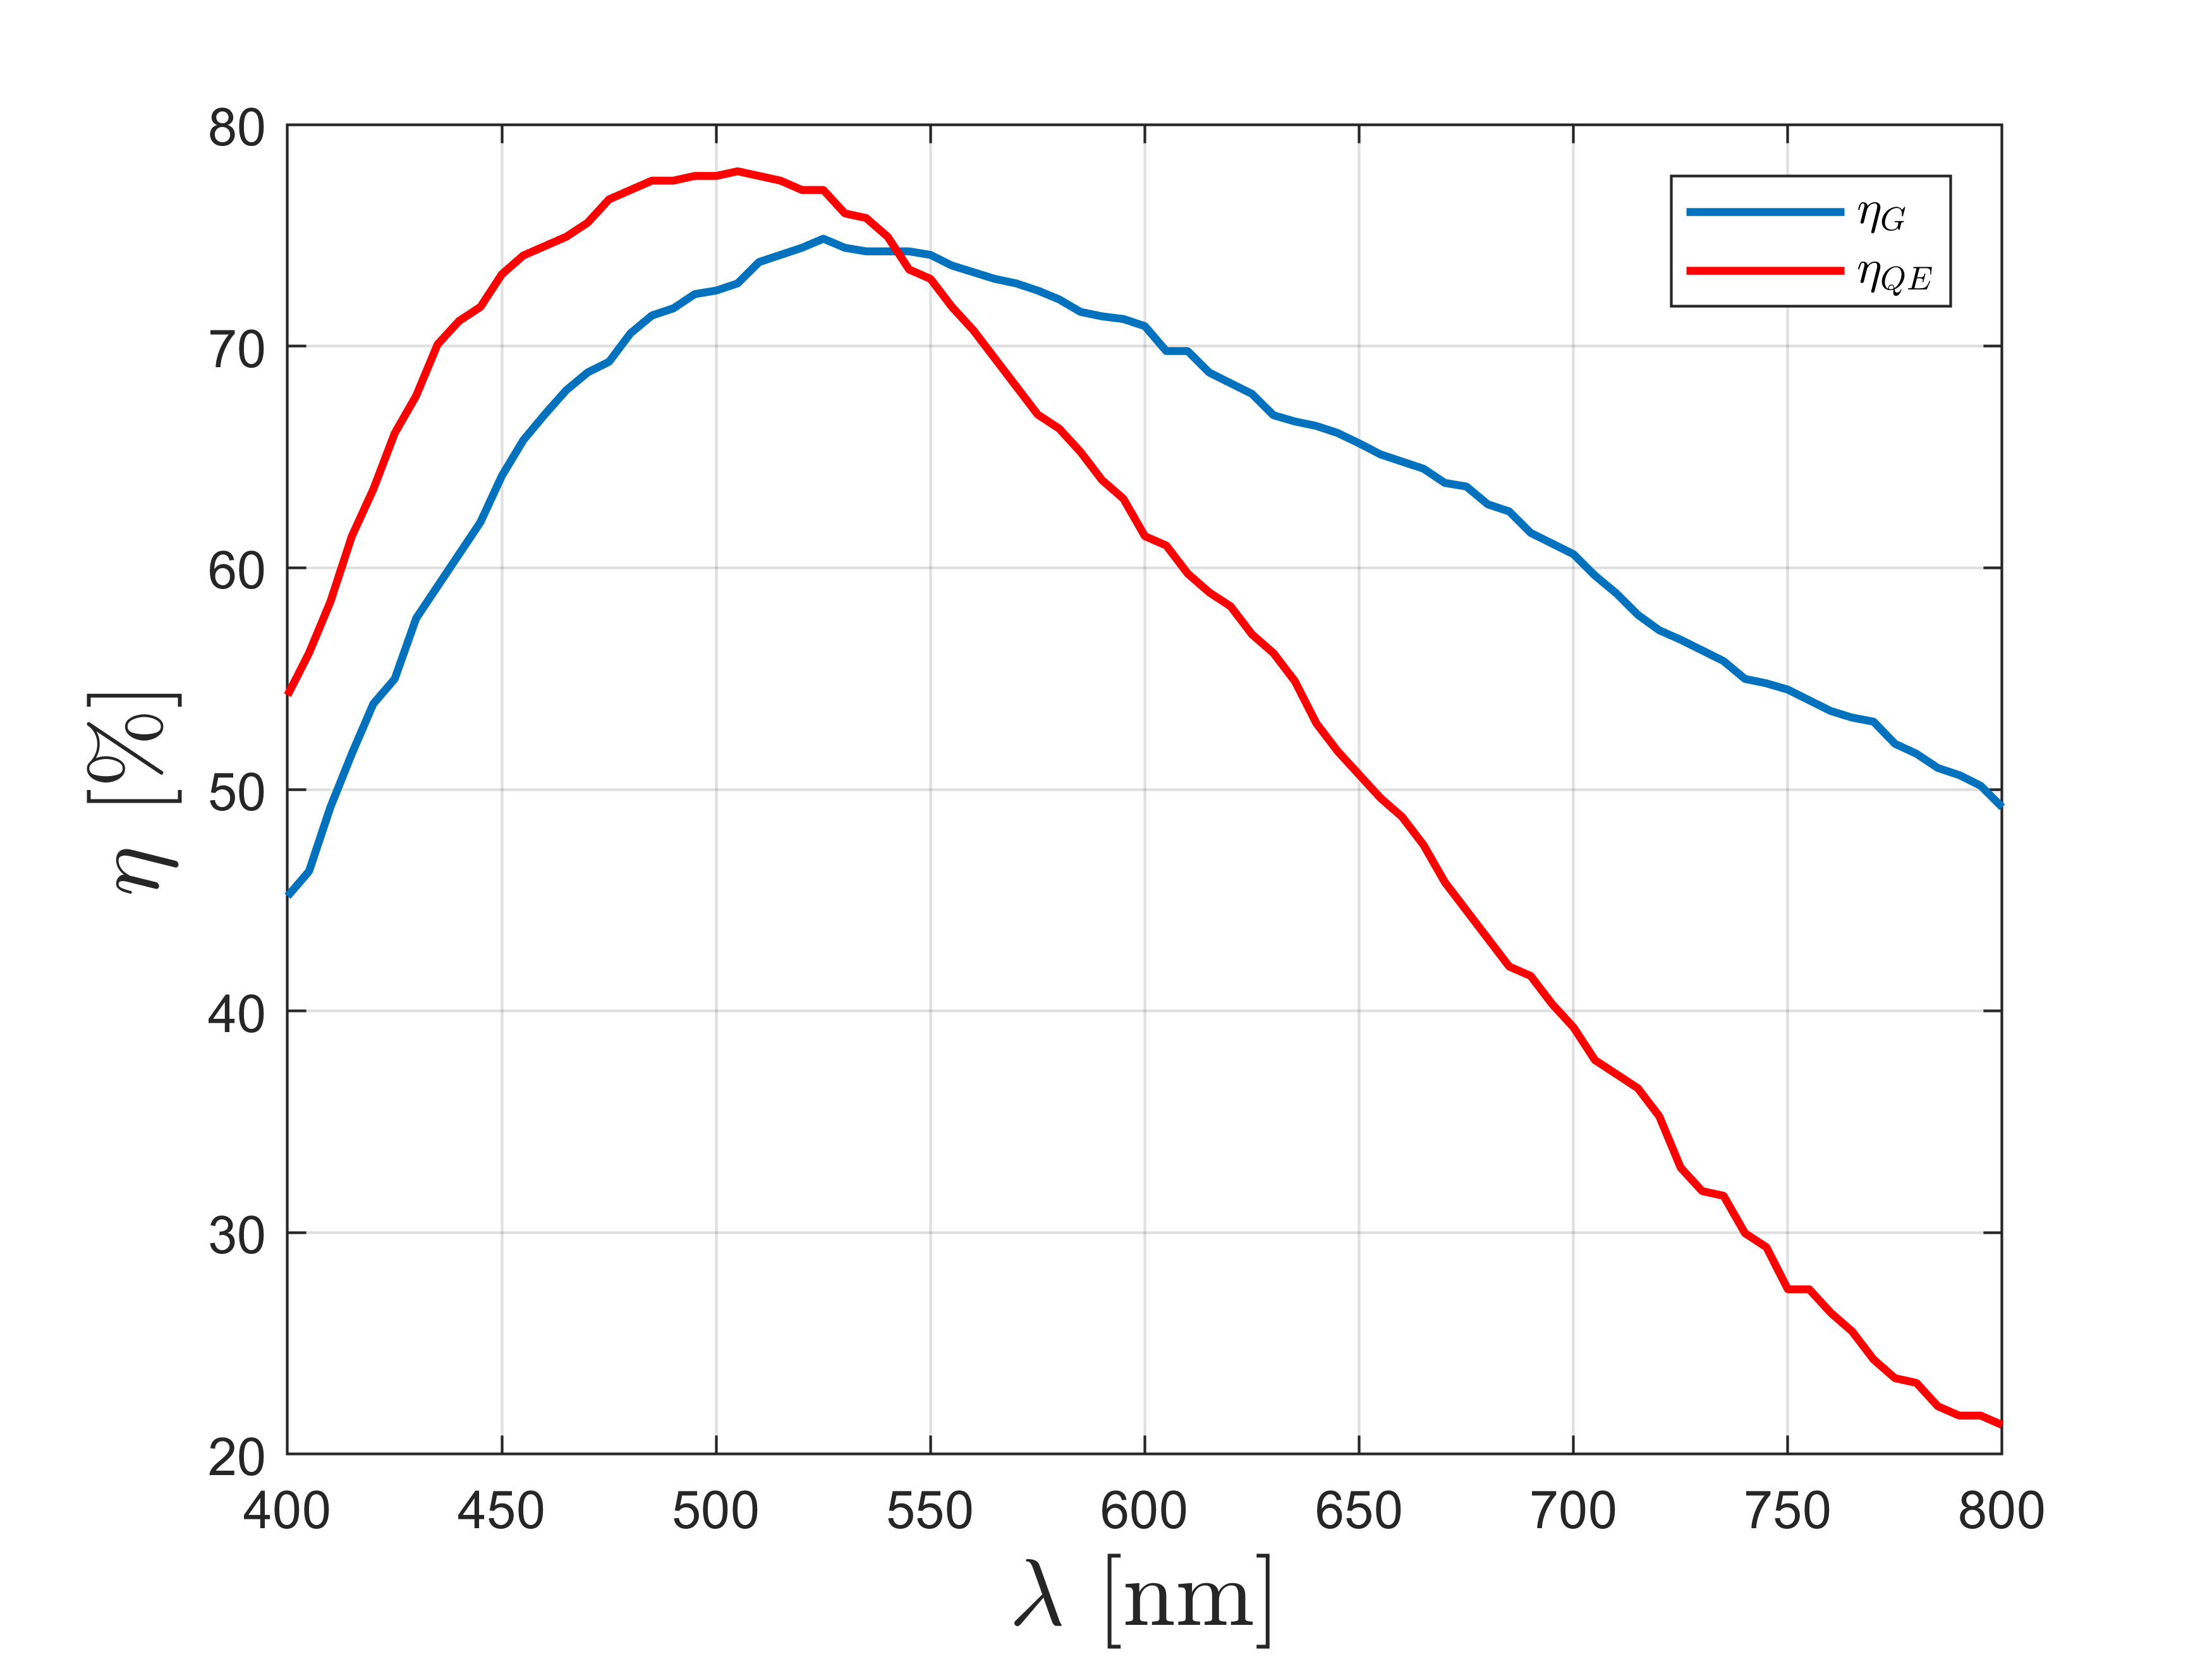
\includegraphics[width=0.4\textwidth]{figs/optical_eff.png}
  \caption{Efficiencies to be expected for grating and HSI sensor SONY IMX249 across the spectral range.}
	\label{fig:optical_eff}
\end{figure}

The effective slit width may be written as
\begin{equation}
\tilde{w}_{\text{slit}} = w_{\text{slit}}\cos\alpha/\cos\beta = 50.8303 \mu m
\end{equation}

Knowing that the pixel size is $p_x=5.86 \mu$m, then the area on the detector per pixel area that are binned twice in spectral direction can be calculated as
\begin{equation}
\tilde{A}_{\text{detector}} = 2\times p_x\times p_x = 2.8826 \times 10^{-10} m
\end{equation}

\noindent Assuming viewing angle $\gamma = 0^{\circ}$, the solid angle of the sensor at Nadir as seen from the earth's surface is
\begin{equation}
\Omega_{\text{aperture}} = \frac{\pi (A_0/2)^2}{r^2} = 4.9087 \times 10^{-16} sr
\end{equation}

\noindent where $r$ is the range and $r=\frac{h}{\cos{\gamma}}$. Entendue is then calculated as
\begin{equation}
E_{\text{aperture}} = \frac{\pi A_0 \cos \alpha}{4 f_0^2}w_{\text{slit}} \tilde{h}_{\text{slit}} = 2.6864e \times 10^{-6} cm^2 sr
\end{equation}
\noindent If we select wavelength $\lambda = 550$ nm, the corresponding number of photo-electrons released in the detector in time $\Delta t = 0.0254 $ seconds is
\begin{equation}
N_{\text{electrons}} = \frac{\pi L \tilde{A}_{\text{detector}} \Delta\lambda \Delta t \eta_{\text{G}} \eta_{\text{OE}} \eta_{\text{QE}} \lambda}{4(f_0/A_0)^2+1)h_{\text{planck}} c} = 6.9082\times10^{4}
\end{equation}
\noindent where $L$ is the irradiance reaching the front lens at ToA for $\lambda = 500$ nm, $h_{\text{planck}}$ and $c$ are Planck's constant and speed of light, respectively. The exposure time $\Delta t = 0.0254 $ determines how much the satellite sees in a movement of $v_{\text{sat}}\times \Delta t =500$ m, i.e. spatial resolution of $\Delta x = \delta x + v_{\text{sat}}\times \Delta t = 693.65$ m at Nadir. Approximately 5-10 \% of total ToA photons consists of water-leaving photons which we are looking for. Of a total of $6.9082\times10^{4}$ photon-electrons, less than $\approx 6.9082\times10^{3}$ water-leaving photon-electrons reach the sensor due to the atmospheric effects shown in Figure \ref{fig:radiance}.  Using the numbers from Tables \ref{tab:optics} and \ref{tab:specs}, the theoretical $SNR$ is calculated as follows,
\begin{equation}
SNR = \frac{N_{\text{electrons}}}{\sqrt{N_{\text{electrons}}+B i_{\text{dark}} \Delta t+B e_{\text{read}}^2}} = 164.8
\end{equation}
\noindent where $B$ is number of binning operations. It is assumed that binning operations are $2\times$ that are incorporated into achieving spectral resolution of $\Delta \lambda=5$ nm. With $SNR$ of $164.8$ at 550 nm, it can be estimated that the $SNR$ of water-leaving radiance will be $\approx 16.4$.

Figure \ref{fig:snr_exposure} shows the sensitivity of SNR to exposure time $\Delta t$. The main compromise here will be between spatial resolution and signal strength due to number of frames taken per second.
\begin{figure}[H]
  \centering
      \includegraphics[width=0.4\textwidth]{figs/snr_exposure.png}
  \caption{SNR vs. exposure time, clearly showing increase in SNR as exposure time becomes longer.}
	\label{fig:snr_exposure}
\end{figure}
However, the sensor saturation capacity limits the collection of photons per pixel due to its dynamic range. The formula for maximum number of intensity counts in Arbitrary Digital Units (ADU) that can be read is
\begin{equation}
I_{\text{max}}=(2^{\text{bit depth}})-1
\end{equation}
\noindent which for a 12-bit ADC gives a maximum of 4095 ADU. The saturation capacity or well depth for the SONY IMX249 is 39541 $e^-$ which means that there are 7.9 $e^-$/ADU. Thus the unbinned and raw practical maximum SNR per pixel is calculated as
\begin{equation}
\tilde{SNR}=\frac{39541}{\sqrt{39541+0.95*0.0254+6.93^2}}= 198.7285
\end{equation} 
\noindent and thus the maximum detectable water-leaving SNR would be about $<19.8$ per pixel. Binning will increase the SNR proportionally with square root number of binned pixels $\sqrt{B}$ or square root number of overlapping pixels $\sqrt{N}$.
\begin{figure}[H]
  \centering
      \includegraphics[width=0.4\textwidth]{figs/snr_exposure_sat.png}
  \caption{SNR where it clearly saturates due to the well depth (saturation capacity).}
	\label{fig:snr_exposure}
\end{figure}

\begin{figure}[htbp]
  \centering
      \includegraphics[width=0.5\textwidth]{figs/slew2.png}
  \caption{\sml at $h=500$ km in two consecutive passes with $\approx 95$ minutes period, where $N+1$ pass shows the target area (same ground point) has moved approximately 1175 km at latitude of $63.11^{\circ}$, resulting a required $\Delta \gamma\approx 64^{\circ}$ from Nadir in cross-track direction.}
	\label{fig:slew2}
\end{figure}
Pointing cross-track would be essential for targets that are off-nadir due to e.g. cloud cover, moving target and sun glint. In order to revisit the target and due to Earth's rotation, the spacecraft not only has to slew along-track but also point in the cross-track direction given that the target area will, in the next pass, have a westwards apparent movement with respect to the orbit. Two cases are to be considered:

\begin{itemize}
\item Figure \ref{fig:slew2} shows the example of the nominal pass where \sml at $h=500$ km flies directly over the $50$ long target, then needing to slew in the cross-track direction from Nadir, it can be shown that for the next pass, \hypso would have to point to $\phi \approx 64^{\circ}$ due to the target having moved $1175$ km westwards after 94.6 min. 

\item If the nominal \sml pass is right in the middle of the target in first and second pass then \sml would have to point to $\phi\approx 45^{\circ}$ wrt. Nadir due to the target having moved $588$ km westwards. 

\end{itemize}
Both the cases can be improved based on altitude selection and independent camera pointing. However, spatial resolution will also worsen, since along-track spatial resolutions are a function of slant range $r=h/\cos\gamma$. The slant range and increases with larger viewing angles hence ground pixels become much larger and resolution of the target worsens. For $\theta=64^{\circ}$, then $r=1140.6$ km, $\delta x=1133.7$ m, $SW =161.57$ km and $\Delta y=132.87$ m. Pointing requirements also need to be strict to avoid considerable motion blur and geometrically inconsistent pixels in the frame, which should typically give less than $100$ m error in order to achieve desired image resolution.

Furthermore, the water-leaving radiance is related to the the phase function (assuming the water radiance is scattered by Lambertian BRDF) i.e.,
\begin{equation}
p(\gamma) = \frac{2}{3\pi^2}\left(\sin\gamma + (\pi-\gamma)\cos\gamma \right)
\end{equation}
\noindent thus the reflected radiance from the water surface scatter and decrease when \hypso views the target at larger angles.

\subsection{Saturation}
One way to avoid green light saturation is to use an amethyst filter (e.g. \url{http://www.koppglass.com/filter-catalog/purple-filter-glass.php}) having a transmission curve that suppresses the green.  Of course green signal is thrown away but at least can potentially improvement is made on the relative blue and red SNR while avoiding saturating the detector, which will likely render the whole frame indistinguishable; at best is to decimate the green part of the hypercube.

\subsection{Stray Light}
Stray light within the spectrograph may dominate the "noise" in the SNR problem. Any photon that does not reach the theoretically perfect place on the photodetector; that is the right row of color and the right column of cross-track location is called stray light. Sources include scattering/refraction from scratch and dig, stria, or cement flaws in the optics, monochromatic (Zernike) aberrations, chromatic aberration, polarization sensitivity, and non-ideal diffraction grating effects including scattering from ruling flaws, low diffraction efficiency (e.g. related to where the un-diffracted light goes), and poor order blocking filter performance. Characterization and correction schemes are given in \cite{Zonga2007}.

\subsection{Atmospheric Correction}
Aerosols, gases, humidity, bubbles etc. distort the spectral response for a HSI. Figure \ref{fig:radiance} shows this effect, where 85-95 $\%$ of photons (depending on wavelength) are coming directly from the atmosphere. Since NIR is absorbed by the atmosphere (and water) more than VIS, many atmospheric corrections are employed using NIR \cite{Corson2011, Patissier2014}.

The advantages and challenges with HSI coastal observations in space are discussed briefly in \cite{Emberton2016}. The water-leaving radiance generally only accounts for around 10-15 \% of the signal that may be observed in space, with the rest of the signal being corrupted by atmospheric and surface/landscape effects, especially for Case 2 waters being mostly coastal waters. It is noted that turbid waters and strong-absorbing aerosols occur in coastal waters which may bring challenges to remote sensing where NIR is necessary for these type of corrections. 700-800 nm may be used to discriminate clouds and land from the open ocean, as well as to map surface vegetation \cite{Emberton2016} such as on Coastal Zone Color Scanner (CZCS), launched by NASA in 1978.

Usage of HSI for high-sediment-loads observations (in VIS-NIR) is investigated by \cite{Lee2016}. Spectral coverage to the shortwave-infrared (SWIR) region is useful for the estimation of suspended particulate matter (SPM) concentrations and for the correction of atmospheric contributions for remote sensing of coastal/in-land turbid waters. \cite{Siegel2000} also concludes with the necessity with NIR bands for proper atmospheric corrections, even for high Chl-a concentrations.

Hyperspectral Imager for the Coastal Ocean (HICO), mounted on ISS and retired in 2014, leveraged data to estimate Chl-a concentration in coastal waters, and was a successor to MEdium Resolution Imaging Spectrometer (MERIS). A further note on this is that it is common knowledge that MERIS superseded MODerate resolution Imaging Spectroradiometer (MODIS) given its band at 708 nm for estimating low-moderate Chl-a concentrations in turbid waters. HICO was a push broom sensor that captured data in the wavelength range 350-1080 nm, with a spectral resolution of 5.73 nm and GSD $\approx 90$m. \cite{Moses2013} presents the radiometric processing results and limitations using red-NIR models, as well as suggestions for future applications of spaceborne HSI in coastal waters. Again, high turbidity renders conventional blue-green algorithms unreliable for estimating Chl-a concentrations. To combat the optical complexity in such cloudy waters, algorithms for red and NIR regions of the spectrum have been recently developed and successfully validated for estimating Chl-a concentration in inland and coastal waters. HICO had problems with the red-NIR spectral range of 700-1080 nm due to contamination by diffracted second-order light in the wavelength range of 350-540 nm, from lack of an optical filter that would block out this second-order light. However there are empirical methods to alleviate this successfully \cite{Li2012}, and by optical design \cite{Fred2017}. The radiometric instability issue should be investigated further including the ability for onboard calibration (latter not possible for HICO). The visible light (400-700 nm) penetrates the water and provides information on water properties and bottom reflectance, and shortwave infrared radiation (700-900 nanometers) is used to correct for atmospheric aerosols and surface reflectance \cite{Corson2011}.

Hyperion, which was launched in 2000, has been used for coastal water studies. However, its SNR (50:1) was
very low \cite{Hu2012}, and the sensor was unreliable in quantitatively estimating water quality parameters due to problems such as radiometric instability \cite{NRC2007}. HICO, on the other hand has high SNR (200:1) over the visible wavelengths \cite{Corson2011}. Even SNR of $>200:1$ is achieved for NIR wavelengths, assuming 5 \% albedo.

Spatial ground resolution of 100 m is recommended in order to characterize ocean coastal waters, and even higher resolution is required for high biodiversity of phytoplankton in certain coastal and inland waters \cite{Emberton2016}. LandSat for instance, "accidentally" proved useful for ocean color due to the high resolution, even though the application was not intended. \cite{Emberton2016} provides an overview of current and previous HSI flights as well as challenges.

Furthermore, \cite{Gitelson2011} presents results using NIR bands for Chl-a concentration estimation from HICO and states that, apart from visible wavelengths for direct chlorophyll observations, shortwave infrared radiation (700-900 nm) is used to correct for atmospheric aerosols and surface reflectance \cite{Corson2011}. It is especially important with these corrections for the retrieval of low-to-moderate Chl-a concentration.

Radiometric resolution datasheets on Sentinel-3 Ocean and Land Colour Instrument (OLCI) exist where the application of each spectral band is indicated\footnote{\url{https://sentinel.esa.int/web/sentinel/user-guides/sentinel-3-olci/resolutions/radiometric}}. OLCI is a push-broom imaging spectrometer with five cameras, where mitigation of sun-glint contamination is done by tilting cameras in westerly direction. Other specs for the OLCI are: swath width of 1270 km, spectral range of 400-1020 nm and spatial sampling of 300 m. From the datasheet it is evident what functionality each of the NIR bands have: 778.75 nm for atmospheric and aerosol corrections; 865 nm for atmospheric and aerosol corrections, clouds, pixel co-registration; 885 nm for water vapour absorption reference band and is the common reference band with SLSTR instrument, also used for vegetation monitoring; 900 nm for water vapour absorption/vegetation monitoring (max. reflectance).

See Fig. \ref{fig:missions_chl} for an overview of usage of the spectral bands in satellite missions.
\begin{figure}[htbp]
  \centering
      \includegraphics[width=0.5\textwidth]{figs/missions_Chl.png}
  \caption{Satellite missions with Multi-spectral Imagers and utilization of each spectral bands \cite{Patissier2014}}
	\label{fig:missions_chl}
\end{figure}
Several other techniques are also envisaged to be investigated in contrast to the standard techniques in atmospheric correction. These involve using analytical algorithms based on the derivatives of the radiative transfer equation, termed as the derivative ratio algorithm \cite{Philpot1991}. A spectral shape algorithm that uses derivatives has been applied to Medium Resolution Imaging Spectrometer (MERIS) imagery that has detected cyanobacterial blooms, with extensive examples in Lake Erie \cite{Wynne2013}. The detection algorithm uses an approximation of the second derivative as a measure of spectral shape around the 681 nm band and has proven that these algorithms prove successful results without compromising the systematic noise in SNR.

\subsection{Calibration}
Suggestions on calibration for HSI testbed to image the following (in order of priority):
\begin{enumerate}
\item	Wavelength calibration - Monochromatic light source, see if we can get the spectral response matching apriori knowledge of spectral band. Determine if sensor output spectral response is shifted from nominal. May use spectral photometer. \ref{fig:calib} shows the 1st wavelength calibration performed on HSI V6. 
\item Keystone characterization
\item Smile characterization
\item Radiometric calibration
\item	Blue sky and characterize the spectral response as above in 1.
\item	Black body source of light. Characterize spatial vs. spectral response. Characterize Quantization Efficiency at different wavelengths. 
\item	Diffuse source of light (e.g. water) - even illumination (not focused images)
\item	Closing the camera cap to characterize dark noise, bias and read-out noise with different in exposure times based on camera specifications.
\item Any source of light (clean room) and subtract the noise to see signal response.
\end{enumerate}

It is important to characterize Quantization Efficiency across wavelengths, edges of spectral range (400-900 nm) have lower quantization efficiency (vignetting). Additional noise comes from microbubbles (Rayleigh scattering) and also needs to be characterized (microbubbles most likely have noise described as random or by Brown distortion model).

One option is to take several images of a track and average those multiple images to estimate the noise in the camera and scene. Eventually one may determine PSNR for image reconstruction, also SNR to characterize image before and after reconstruction.

\begin{figure}[htbp]
  \centering
      \includegraphics[width=0.45\textwidth]{figs/calibration.png}
  \caption{1st Wavelength calibration using the Imaging Source IMX174LLJ camera head. Source spectrum is office roof illuminated by an OSRAM FQ 54W/830 HO Fluorescence tube}
	\label{fig:calib}
\end{figure}
